\documentclass{beamer}
\usepackage{moreverb} 
\usepackage{listings}
\usepackage{mflogo}
% imprimir
% \documentclass[handout]{beamer} 
% \usepackage{pgfpages}
% \pgfpagesuselayout{4 on 1}[a4paper,landscape,border shrink=5mm]

\mode<presentation> {
  \usetheme{Warsaw}
  \setbeamercovered{opaque}
}

\usebackgroundtemplate{\includegraphics[width=\paperwidth]{format/libresoft-bg.png}}
\usepackage[spanish]{babel}
\usepackage[utf8]{inputenc}
\usepackage{graphics}
\usepackage{amssymb} % Simbolos matematicos

%% Metadatos del PDF.
\hypersetup{  
  pdftitle={Free Unix-like Operating Systems},
  pdfauthor={Miguel Vidal},
  pdfcreator={GSyC/Libresoft},
  pdfproducer=PDFLaTeX,
  pdfsubject={Master on Free Software},
}
%%

\defbeamertemplate*{footline}{shadow theme}
{%
  \leavevmode%
  \hbox{\begin{beamercolorbox}[wd=.5\paperwidth,ht=2.5ex,dp=1.125ex,leftskip=.1cm plus1fil,rightskip=.2cm]{author in head/foot}%

\includegraphics[scale=0.40]{format/cc-by-80x15.png} \hspace{0.05cm}
	Miguel Vidal / Jose Castro
  \end{beamercolorbox}%
  \begin{beamercolorbox}[wd=.5\paperwidth,ht=2.5ex,dp=1.125ex,leftskip=.3cm,rightskip=.3cm plus1fil]{title in head/foot}%
    \usebeamerfont{title in head/foot}\insertshorttitle%
    \hspace{2cm} \usebeamerfont{author in head/foot}\insertframenumber\,/\,\inserttotalframenumber\hfill
  \end{beamercolorbox}}%
  \vskip0pt%
}


\begin{document}

\title{Free Unix-like Operating Systems}
\subtitle{System Integration}
% \institute{\texttt{http://gsyc.urjc.es/\~{}mvidal} \\ Twitter: \texttt{@mvidallopez}}
\author{Miguel Vidal, Jose Castro} 
\date{\footnotesize{Master on Free Software \\ March 23rd, 2012}}
\author{Miguel Vidal \hspace{1cm} Jose Castro \\
\hspace{0.5mm} {\tiny Twitter: @mvidallopez \hspace{1.1cm}Twitter: @jfcastroluis}
}


\frame{
\maketitle
\begin{center}

\includegraphics[width=6cm]{format/gsyc-urjc}
\end{center}
}

%% License slide
\begin{frame}
  \vspace{2cm}
  \begin{flushright}
    {\small \copyright{} 2010-2012 Miguel Vidal, Jose Castro} \\
%    \vspace{0.25cm}
    \medskip
    {\scriptsize This work is licensed under \\ a Creative Commons Attribution 3.0 License}
%    \vspace{0.10cm}
  \end{flushright}
  \begin{flushright}
    \href{http://creativecommons.org/licenses/by/3.0/es}{\includegraphics[width=2cm]{format/cc-by.png}} \\
    {\tiny \url{http://creativecommons.org/licenses/by/3.0}}
  \end{flushright}
\end{frame}%%

\usebackgroundtemplate{}

\AtBeginSection[]
{
\begin{frame}<beamer>
\begin{center}
{\huge \insertsection}
\end{center}
\end{frame}
}


\AtBeginSubsection[]
{
  \begin{frame}<beamer>{Índice}
    \tableofcontents[currentsection,currentsubsection]
  \end{frame}
}

%%

\normalsize


%%%%%%%%%%%%%%%%%%%%%%%%%%%%%%%%%%%%%%%%%%%%%%%%%%%%%%%%%%%%%%%%%%%%%%%

\section{Qué es Unix}
\subsection{Qué es Unix}
\begin{frame}
\frametitle{¿Qué es Unix? (1)}

\begin{itemize}
\item Sistema operativo multitarea y multiusuario. 
\item Muy portable (C). 
\item No hay un solo Unix, sino numerosas ramas. 
\item Probablemente cientos de variantes a lo largo de más de 40 años de historia.
\end{itemize}

\end{frame}

%%%%%%%%%%%%%%%%%%%%%%%%%%%%%%%%%%%%%%%%%%%%%%%%%%%%%%%%%%%%%%%%%%%%%%%

\begin{frame}
\frametitle{¿Qué es Unix? (y 2)}

\begin{itemize}
\item Se desarrolla al tiempo que Internet y es la base de la tecnología internet (TCP/IP).
\item Los Unices comparten una estructura común, compatibilidad binaria (ELF), POSIX shell, servicios y utilidades como awk, echo, ed, vi y muchas otras.
\end{itemize}

\end{frame}


%%%%%%%%%%%%%%%%%%%%%%%%%%%%%%%%%%%%%%%%%%%%%%%%%%%%%%%%%%%%%%%%%%%%%%%
\subsection{La marca Unix}
\begin{frame}
\frametitle{\textsc{UNIX\texttrademark}: La marca Unix (1)}

\begin{itemize}
\item Oficialmente \textsc{UNIX\texttrademark} es una \alert{marca registrada}, desde 1996 controlada por el consorcio neutral Open Group. 
\item Formado por más de 300 organizaciones, entre ellas grandes corporaciones (Oracle, HP, IBM, Fujitsu...)
\item El Open Group concede el uso de la marca a quienes cumplen con la Single UNIX Specification (SUS).
\item El certificado no requiere el código fuente, por lo que pueden no tener código en común ni ser derivados del Unix original.
\end{itemize}

\end{frame}

%%%%%%%%%%%%%%%%%%%%%%%%%%%%%%%%%%%%%%%%%%%%%%%%%%%%%%%%%%%%%%%%%%%%%%%
\begin{frame}
\frametitle{La marca Unix (2)}

\begin{itemize}
\item Para los modelos de desarrollo libres, la especificación es demasiado cara e insostenible.
\item GNU: \alert{G}NU's \alert{N}ot \alert{U}nix. 
\item \alert{Unix-like} (``tipo Unix''), ``*nix'' o ``Un*x'': SOs que no cumplen la especificación, para sortear el problema del uso de la marca (aunque no gusta a sus propietarios).
\item FreeBSD tiene una certificación ``C99'' (ISO 9899:1999) conforme POSIX, que cumple en gran parte con SUS.
\item Linux usa una especificación LSB (Linux Standard Base), muy próximo a POSIX y que más o menos siguen todas las distribuciones. 
\end{itemize}

\end{frame}


%%%%%%%%%%%%%%%%%%%%%%%%%%%%%%%%%%%%%%%%%%%%%%%%%%%%%%%%%%%%%%%%%%%%%%%

\begin{frame}
\frametitle{La marca Unix (y 3)}

\begin{itemize}
\item El uso de la marca cuesta dinero y solo los Unixes comerciales (y privativos) tienen la certificación: AIX, HP-UX, SCO, Solaris, Mac OS X, IRIX...
\item Comparten POSIX shell, servicios y utilidades como \texttt{awk}, \texttt{echo}, \texttt{ed}, \texttt{vi} y muchas otras.
\item No tienen por qué proceder del Unix original.
\end{itemize}

\end{frame}


%%%%%%%%%%%%%%%%%%%%%%%%%%%%%%%%%%%%%%%%%%%%%%%%%%%%%%%%%%%%%%%%%%%%%%%
\subsection{Clases de Unix}
\begin{frame}
\frametitle{Clases de Unix}

Clasificación propuesta por Eric Raymond:

\begin{itemize}
\item \alert{Unix genético}: descendientes del código Unix original de AT\&T (muchos Unix comerciales y los actuales BSD).
\item \alert{Unix de marca}: los que tienen la especificación SUS (Solaris, AIX, HP-UX, MacOS X...). Solo estos pueden usar \alert{legalmente} el nombre \textsc{UNIX\texttrademark}.
\item \alert{Unix funcional}: los que se acercan a la especificación POSIX o se comportan de forma consistente como Unix (como Linux o Minix), pero no poseen la marca ni descienden del código del Unix original.
\end{itemize}

\end{frame}


%%%%%%%%%%%%%%%%%%%%%%%%%%%%%%%%%%%%%%%%%%%%%%%%%%%%%%%%%%%%%%%%%%%%%%%

% \begin{frame}
% \frametitle{El surgimiento de Unix}

% El nacimiento de Unix fue una auténtica revolución del software:

% \begin{itemize}

% \item 1969: Ken Thompson inventó Unix (mismo año que Arpanet).
% \item Surge de los deshechos de Multics, en AT\&T (Bell Labs). 
% \item Dennis Ritchie inventa un nuevo lenguaje llamado C para usarlo en el Unix de Thompson. 
% \item Primer sistema operativo portable y modular (KISS), frente a anteriores sistemas incompatibles y costosos.
% \item Se extiende rápidamente y de forma no oficial por AT\&T. Y por Arpanet (hardware distinto, gracias a C).
% \item Acuerdo judicial (\textit{antitrust}) de 1956 impide a AT\&T comercializar Unix: debe licenciarlo (con fuentes) a quien se lo solicite.

% \end{itemize}

% \end{frame}


%%%%%%%%%%%%%%%%%%%%%%%%%%%%%%%%%%%%%%%%%%%%%%%%%%%%%%%%%%%%%%%%%%%%%%%

\begin{frame}
% \frametitle{Historia de Unix}


\begin{figure}[h]

\begin{center}
  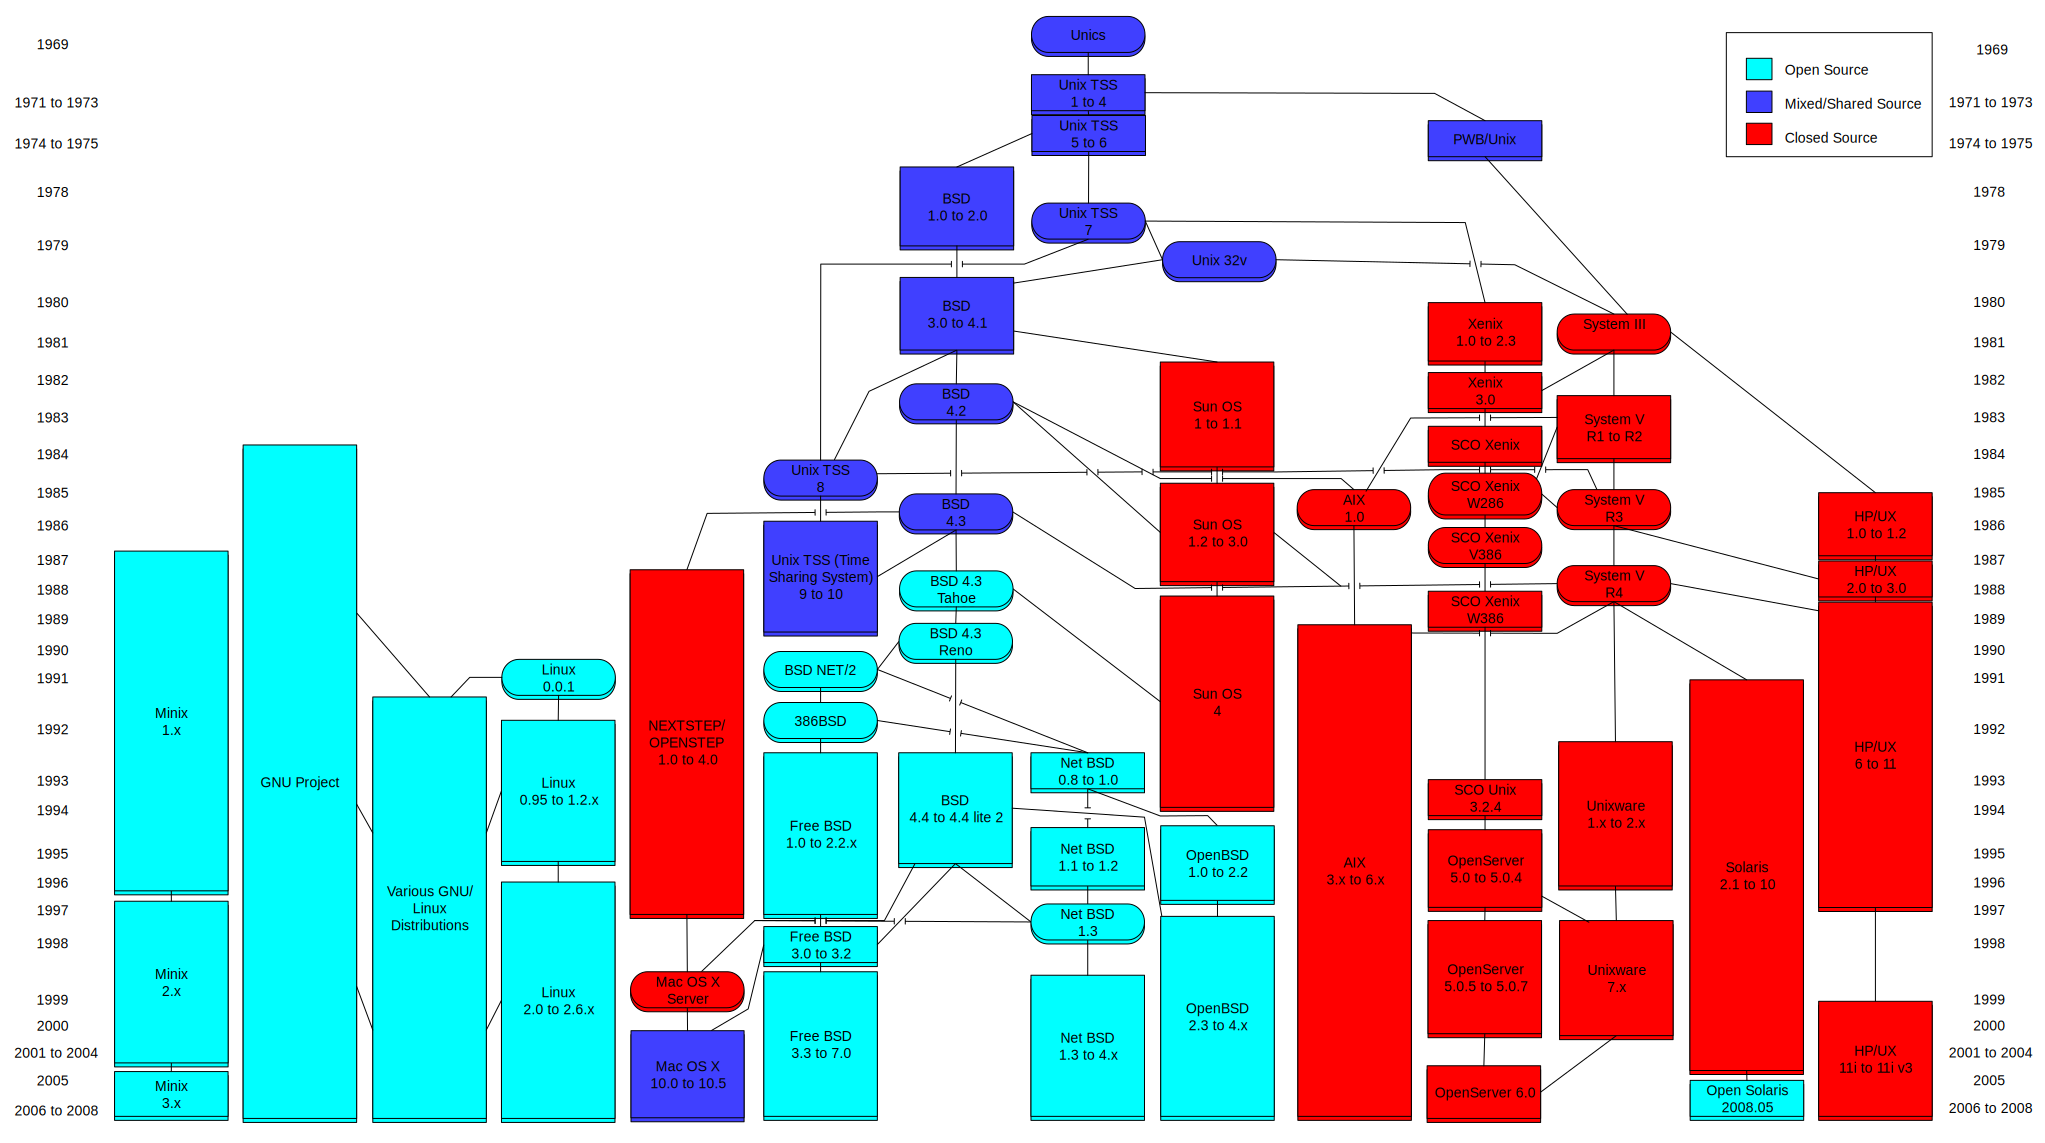
\includegraphics[height=2.7in]{figs/Unix_history-simple.png}
  \caption{{\footnotesize Historia de Unix. \textit{Fuente: Wikipedia}}}
\end{center}
\end{figure}


\end{frame}

%%==================================================================
%%---------------------------------------------------------------


%%%%%%%%%%%%%%%%%%%%%%%%%%%%%%%%%%%%%%%%%%%%%%%%%%%%%%%%%%%%%%%%%%%%%%
\section{Variantes de Unix}
\subsection{Variantes de Unix}
\begin{frame}
\frametitle{Variantes de Unix}

Dos grandes variantes históricas:

\begin{itemize}
\item System V
\item BSD
\end{itemize}

\end{frame}

%%%%%%%%%%%%%%%%%%%%%%%%%%%%%%%%%%%%%%%%%%%%%%%%%%%%%%%%%%%%%%%%%%%%%%

\begin{frame}
\frametitle{Variantes de Unix (2)}

\begin{itemize}
\item Algunos sistemas mantenían las dos versiones en paralelo (con comandos, directorios, páginas \texttt{man} y librerías distintos). A estas variantes se les llamaba \alert{``universos''}.
\item Esta división era problemática a la hora de portar aplicaciones y mantener los sistemas.
\item Cada universo fue adoptando lo mejor del otro. 
\item En 1988, se produce una fusión entre ambas: \alert{System R4}. 
\item Hoy día quedan reminiscencias en algunos sistemas, que tienen un directorio separado con los comandos estilo BSD o System V.
\end{itemize}


\end{frame}


%%%%%%%%%%%%%%%%%%%%%%%%%%%%%%%%%%%%%%%%%%%%%%%%%%%%%%%%%%%%%%%%%%%%%%%
\subsection{Universos de Unix}
\begin{frame}
% \frametitle{Los dos grandes ``universos'' de Unix}


\begin{figure}[h]

\begin{center}
  \includegraphics[height=2.60in]{figs/Unix_history.png}
  \caption{{\footnotesize Los dos grandes ``universos'' de Unix. \textit{Fuente: Wikipedia}}}
\end{center}
\end{figure}


\end{frame}

%%%%%%%%%%%%%%%%%%%%%%%%%%%%%%%%%%%%%%%%%%%%%%%%%%%%%%%%%%%%%%%%%%%%%%%

\begin{frame}
\frametitle{Un ejemplo: el comando `\texttt{ps}' en Linux}

\begin{figure}[h]

\begin{center}
  \includegraphics[height=2.4in]{figs/ps.png} \\
\caption{{\footnotesize Comando \texttt{ps} en Linux.}}
\end{center}
\end{figure}

\end{frame}

%%%%%%%%%%%%%%%%%%%%%%%%%%%%%%%%%%%%%%%%%%%%%%%%%%%%%%%%%%%%%%%%%%%%%%%

\begin{frame}
\frametitle{Un ejemplo: el comando `\texttt{ps}' en Linux}

\begin{figure}[h]

\begin{center}
  \includegraphics[height=1.5in]{figs/ps-2.png}
\caption{{\footnotesize Comando \texttt{ps} en Linux.}}
\end{center}
\end{figure}

\end{frame}


%%%%%%%%%%%%%%%%%%%%%%%%%%%%%%%%%%%%%%%%%%%%%%%%%%%%%%%%%%%%%%%%%%%%%%

% \begin{frame}
% \frametitle{System V R4}


% \begin{itemize}

% \item Promovida por Sun, USL y Xenix
% \item De BSD: TCP/IP, sockets, ufs, csh
% \item De SunOS: NFS, RPC, OpenWindows...
% \item De Xenix: drivers para x86, compatibilidad binaria con Xenix
% \item Muchas versiones comerciales (privativas de los 90 se basaron en SVR4: Solaris, SCO, HP, SGI...
% \item OpenSolaris: única versión libre de SVR4.

% \end{itemize}

% \end{frame}



%%%%%%%%%%%%%%%%%%%%%%%%%%%%%%%%%%%%%%%%%%%%%%%%%%%%%%%%%%%%%%%%%%%%%%
\section{Unix libres}
\subsection{Los BSD}
\begin{frame}
\frametitle{Unixes libres: los BSD}

Todos derivan del BSD Unix original. Principales proyectos:

\begin{itemize}
\item FreeBSD (1993)
\item NetBSD (1993)
\item OpenBSD: fork de NetBSD (1995)
\item DragonFly BSD (2004)
\item PC-BSD

\end{itemize}

Cada uno tiene, a su vez, numerosas variantes.

\pause

\begin{center}
Lista de SOs basados en BSD: 
\begin{small}
\url{http://en.wikipedia.org/wiki/List_of_BSD_operating_systems}
\end{small}
\end{center}

\end{frame}

%%%%%%%%%%%%%%%%%%%%%%%%%%%%%%%%%%%%%%%%%%%%%%%%%%%%%%%%%%%%%%%%%%%%%%

\begin{frame}
\frametitle{Unixes libres: FreeBSD}

\begin{itemize}
\item Es el BSD más popular. Rápido y optimizado para plataformas i386/amd64.
\item Rápida incorporación de mejoras. Buenas versiones de escritorio.
\item Su kernel incorpora un sistema de virtualización ligera muy apreciado: las \textit{jails}
\item Ha portado el sistema de ficheros ZFS de OpenSolaris.
\end{itemize}

\end{frame}

%%%%%%%%%%%%%%%%%%%%%%%%%%%%%%%%%%%%%%%%%%%%%%%%%%%%%%%%%%%%%%%%%%%%%%

\begin{frame}
\frametitle{Unixes libres: OpenBSD (1)}

\begin{itemize}
\item Se concentra en la corrección, seguridad proactiva, portabilidad (17 arquitecturas) y libertad.
\item Código del sistema base auditado, características de seguridad y criptografía integradas. 
\item PF: el mejor firewall
\item OpenSSH: la mejor shell segura.
\item No intenta estar a la última, prioriza la sencillez y la estabilidad.
\end{itemize}


\end{frame}

%%%%%%%%%%%%%%%%%%%%%%%%%%%%%%%%%%%%%%%%%%%%%%%%%%%%%%%%%%%%%%%%%%%%%%

\begin{frame}
\frametitle{Unixes libres: OpenBSD (y 2)}


\begin{itemize}
\item Comunidad preocupada por la libertad del software: no NDAs, no blobs, la licencia más permisiva de todas (ISC). 
\item La calidad de su documentación es legendaria.
\item Introdujo el uso de CVS y el registro de \textit{commits}, luego adoptado por todas las comunidades de software libre. 
\item Ha logrado que muchos fabricantes de tarjetas de red liberen especificaciones de sus drivers.

\end{itemize}

\end{frame}


%%%%%%%%%%%%%%%%%%%%%%%%%%%%%%%%%%%%%%%%%%%%%%%%%%%%%%%%%%%%%%%%%%%%%%

\begin{frame}
\frametitle{Unixes libres: NetBSD}

\begin{itemize}
\item Orientado a la portabilidad: se propone funcionar en tantas arquitecturas de hardware como sea posible.
\item Como todos los BSD actuales, deriva del BSD-lite del CSGR de Berkeley.
\item Es el antecesor de OpenBSD.
\end{itemize}

\end{frame}

%%%%%%%%%%%%%%%%%%%%%%%%%%%%%%%%%%%%%%%%%%%%%%%%%%%%%%%%%%%%%%%%%%%%%%

\begin{frame}
\frametitle{Unixes libres: DragonFly BSD}

\begin{itemize}
\item Derivado de FreeBSD 4.8 (2003). 
\item Orientado a la gestión de concurrencia y SMP.
\item Híbrido entre kernel monolítico y microkernel.
\item Inspirado en ideas de AmigaOS.
\end{itemize}

\end{frame}


%%%%%%%%%%%%%%%%%%%%%%%%%%%%%%%%%%%%%%%%%%%%%%%%%%%%%%%%%%%%%%%%%%%%%%
\subsection{OpenSolaris/illumos y derivados}
%%%%%%%%%%%%%%%%%%%%%%%%%%%%%%%%%%%%%%%%%%%%%%%%%%%%%%%%%%%%%%%%%%%%%%

\begin{frame}
\frametitle{Ventajas de OpenSolaris/illumos}

\begin{itemize}
\item \alert{Service Manager Facility} (SMF): sistema de gestión de servicios que reemplaza a los scripts init.d (SVR4).
\item \alert{ZFS} (Zettabyte File System): sistema de ficheros nativo de OpenSolaris que provee administración simplificada, cifrado transparente, volúmenes lógicos, snapshots y \textit{copy-on-write}, chequeo de integridad, RAID-Z, NAS/SAN y una escalabilidad inmensa. Bajo licencia CDDL, por tanto no compatible con Linux (hay \textit{workarounds}).
\item \alert{DTrace:} Herramienta de instrumentación para depurar problemas y errores en el SO y sus aplicaciones en producción y en tiempo real, sin apenas impacto.
\end{itemize}

\end{frame}

%%%%%%%%%%%%%%%%%%%%%%%%%%%%%%%%%%%%%%%%%%%%%%%%%%%%%%%%%%%%%%%%%%%%%%%

\begin{frame}
\frametitle{Ventajas de OpenSolaris/illumos (2/2)}

\begin{itemize}
\item \alert{Solaris Containers} (aka \alert{Zonas}): virtualización ligera. Entornos aislados con una sola instancia del SO. Equivalente a las \textit{jails} de FreeBSD.
\item \alert{LDOMs}: Paravirtualización para arquitectura Sparc (estilo Xen, pero con las ventajas del soporte multi-hilo de las CPUs Sparc).
\item Crossbow: virtualización de redes y recursos para virtualizar el stack completo y las NICs alrededor de cualquier servicio 
\item \alert{KVM:} sistema de virtualización completa (hardware) portado del kernel Linux.
\end{itemize}

\end{frame}

%%%%%%%%%%%%%%%%%%%%%%%%%%%%%%%%%%%%%%%%%%%%%%%%%%%%%%%%%%%%%%%%%%%%%%%

\begin{frame}
\frametitle{Unixes libres: derivados de OpenSolaris}

Principales proyectos:

\begin{itemize}
\item \alert{OpenSolaris}: código base del privativo Solaris 11.
\item \alert{illumos}: fork libre del código de OpenSolaris.
\item \alert{Nexenta OS}: distro basada en illumos y Ubuntu para servidores (GNU \textit{userland}).
\item \alert{OpenIndiana}: distro basada en illumos.
\item \alert{SmartOS}: distro basada en illumos para servidores.
\end{itemize}

\end{frame}

%%%%%%%%%%%%%%%%%%%%%%%%%%%%%%%%%%%%%%%%%%%%%%%%%%%%%%%%%%%%%%%%%%%%%%

\begin{frame}
\frametitle{Derivados de OpenSolaris: SmartOS}

\begin{itemize}
\item Distribución para servidores basada en illumos.
\item Patrocinada por Joyent.
\item Han portado KVM (virtualización de Linux) al kernel de illumos (Solaris).  
\end{itemize}

\end{frame}

%%%%%%%%%%%%%%%%%%%%%%%%%%%%%%%%%%%%%%%%%%%%%%%%%%%%%%%%%%%%%%%%%%%%%%

\begin{frame}
\frametitle{Derivados de OpenSolaris: OpenIndiana}

\begin{itemize}
\item Distribución para escritorio.
\item Auspiciada por la Fundación illumos.
\item Hereda el sistema de paquetes (IPS) y el espíritu de OpenIndiana de Sun (sencillo instalador, Gnome, etc.).
\item También hay versión para servidor.
\end{itemize}

\end{frame}


%%%%%%%%%%%%%%%%%%%%%%%%%%%%%%%%%%%%%%%%%%%%%%%%%%%%%%%%%%%%%%%%%%%%%%
\subsection{Linux}

\begin{frame}
\frametitle{Unixes libres: Linux (1)}

\begin{itemize}
\item Linux es un kernel escrito desde cero. 
\item Es un clon, no un derivado de Unix: pero Dennis Ritchie lo considera un ``Unix de facto''.
\item El proyecto lo inicia Linus Torvalds en 1991, y \textit{just for fun}
\item Incorpora aspectos de las variantes System V y BSD. 
\item Contiene mucho software con origen BSD.
\end{itemize}

\end{frame}

%%%%%%%%%%%%%%%%%%%%%%%%%%%%%%%%%%%%%%%%%%%%%%%%%%%%%%%%%%%%%%%%%%%%%%
\begin{frame}
\frametitle{Unixes libres: Linux (2)}

\begin{itemize}
\item Modelo bazar: desde que liberó la primera versión (0.01) se van uniendo cientos de desarrolladores en un esquema innovador (\textit{release early, release often}).
\item Se adopta la licencia GPLv2.
\item Marzo 1994: versión 1.0
\end{itemize}

\end{frame}



%%%%%%%%%%%%%%%%%%%%%%%%%%%%%%%%%%%%%%%%%%%%%%%%%%%%%%%%%%%%%%%%%%%%%%

\begin{frame}
\frametitle{Unixes libres: Linux (y 3)}

\begin{itemize}

\item Debian y derivados: Ubuntu, Knoppix
\item Red Hat y derivados: RHEL, CentOS, Fedora
\item Gentoo y derivados: Sabayon
\item Ubuntu y derivados: Xubuntu, Kubuntu, Edubuntu, gnewSense, Chrome OS, distros regionales (Guadalinex, LliureX)...
\item Mandriva, SuSE, Slackware...

\end{itemize}

\pause

\begin{center}
Lista de distribuciones Linux: 
\begin{small}
\url{http://en.wikipedia.org/wiki/List_of_Linux_distributions}
\end{small}
\end{center}


\end{frame}

%%%%%%%%%%%%%%%%%%%%%%%%%%%%%%%%%%%%%%%%%%%%%%%%%%%%%%%%%%%%%%%%%%%%%%

\begin{frame}
\frametitle{Promiscuidad de los Unixes libres}

Mezclas de proyectos y código \alert{solo} posible con el software libre:

\begin{itemize}

\item Debian kFreeBSD (kernel FreeBSD en Debian)
\item FreeBSD + ZFS
\item Gentoo/*BSD: \textit{userland} GNU manejado por Portage (el árbol de paquetes) con un kernel \{Net,Free,Open\}BSD.
\item Nexenta: Kernel Solaris y \textit{userland} estilo Ubuntu/Debian (paquetes deb, dpkg y apt).
\item SmartOS: KVM + illumos.
\end{itemize}

\end{frame}


%%%%%%%%%%%%%%%%%%%%%%%%%%%%%%%%%%%%%%%%%%%%%%%%%%%%%%%%%%%%%%%%%%%%%%
\subsection{El caso de MacOS X}
\begin{frame}
\frametitle{El caso de MacOS X}

\begin{itemize}
\item En 1997, Apple Computer refunda su sistema operativo a partir de NeXTSTEP. 
\item NeXTSTEP es un SO privativo desarrollado por NeXT a finales de los 80 y primeros 90. 
\item El núcleo del SO está basado en BSD y en el kernel Mach: pasó a llamarse Darwin después de que Apple lo adquiriera. 
\item Darwin es casi todo software libre (Apple Public Source License), pero Mac OS X \alert{NO} lo es.
\item Darwin y Mac OS X son el sistema Unix más usado en el mercado de los sistemas de escritorio. 
\end{itemize}

\end{frame}

%%%%%%%%%%%%%%%%%%%%%%%%%%%%%%%%%%%%%%%%%%%%%%%%%%%%%%%%%%%%%%%%%%%%%%
% \section{Referencias}
\begin{frame}
\frametitle{Referencias}

\begin{itemize}
\item \textsc{Marshall Kirk McKusick}, ``Twenty Years of Berkeley Unix'', en \textit{Open Sources: Voices from the Open Source Revolution}, O'Reilly, 1999.
\url{http://oreilly.com/openbook/opensources/book/kirkmck.html} 
\textsc{Peter H. Salus} \textit{A Quarter Century of UNIX}. Reading, MA: Addison-Wesley, 1994.
\item \textsc{Peter H. Salus} ``A brief history of System Administration'', pp. 1264-1273 en \textit{ULSAH}, Evi Nemeth et al., Prentice-Hall, 2010.

\end{itemize}

\end{frame}


%%%%%%%%%%%%%%%%%%%%%%%%%%%%%%%%%%%%%%%%%%%%%%%%%%%%%%%%%%%%%%%%%%%%%%

\frame{
\maketitle
\begin{center}

\includegraphics[width=6cm]{format/gsyc-urjc}
\end{center}
}


\end{document}

%%==================================================================
%%---------------------------------------------------------------


